\PassOptionsToPackage{quiet}{fontspec}
\documentclass[oneside]{fdmthesis2023}
\fdusetup{
  style = {
    % fullwidth-stop    =  mapping, % 中文全角句点向全角化英文半角句点的映射
    hyperlink-color   =  classic,
  },
  info = {
    author            = {无名氏},
    date / year       = { 2023 },
    student-id        = {19300180999},
    department        = {数学科学学院},
    major             = {数学与应用数学},
    supervisor        = {有名氏},
    supervisor-title  = {院士},
    supervisor-unit   = {复旦大学数学科学学院物理化学系},
    title             = {复旦大学数学科学学院本科毕业论文\LaTeX 模板(2023年版)},
    title-breakline   = {{复旦大学数学科学学院\\本科毕业论文\LaTeX 模板(2023年版)}},
    keywords          = {甲, 乙, 丙},
    keywords-english  = {A, B, C},
  },
}

\theoremstyle{definition}
  \newtheorem{definition}{定义}[chapter]
\theoremstyle{plain}
  \newtheorem{theorem}[definition]{定理}
  \newtheorem{axiom}[definition]{公理}
  \newtheorem{lemma}[definition]{引理}
  \newtheorem{proposition}[definition]{命题}
  \newtheorem{corollary}[definition]{推论}
\theoremstyle{remark}
  \newtheorem{remark}{注}[chapter]
\def\theequation{\arabic{chapter}.\arabic{equation}}
\def\thedefinition{\arabic{chapter}.\arabic{definition}}

% 到时候用来添加封面二和封面三
% \renewcommand{\makecoverii}{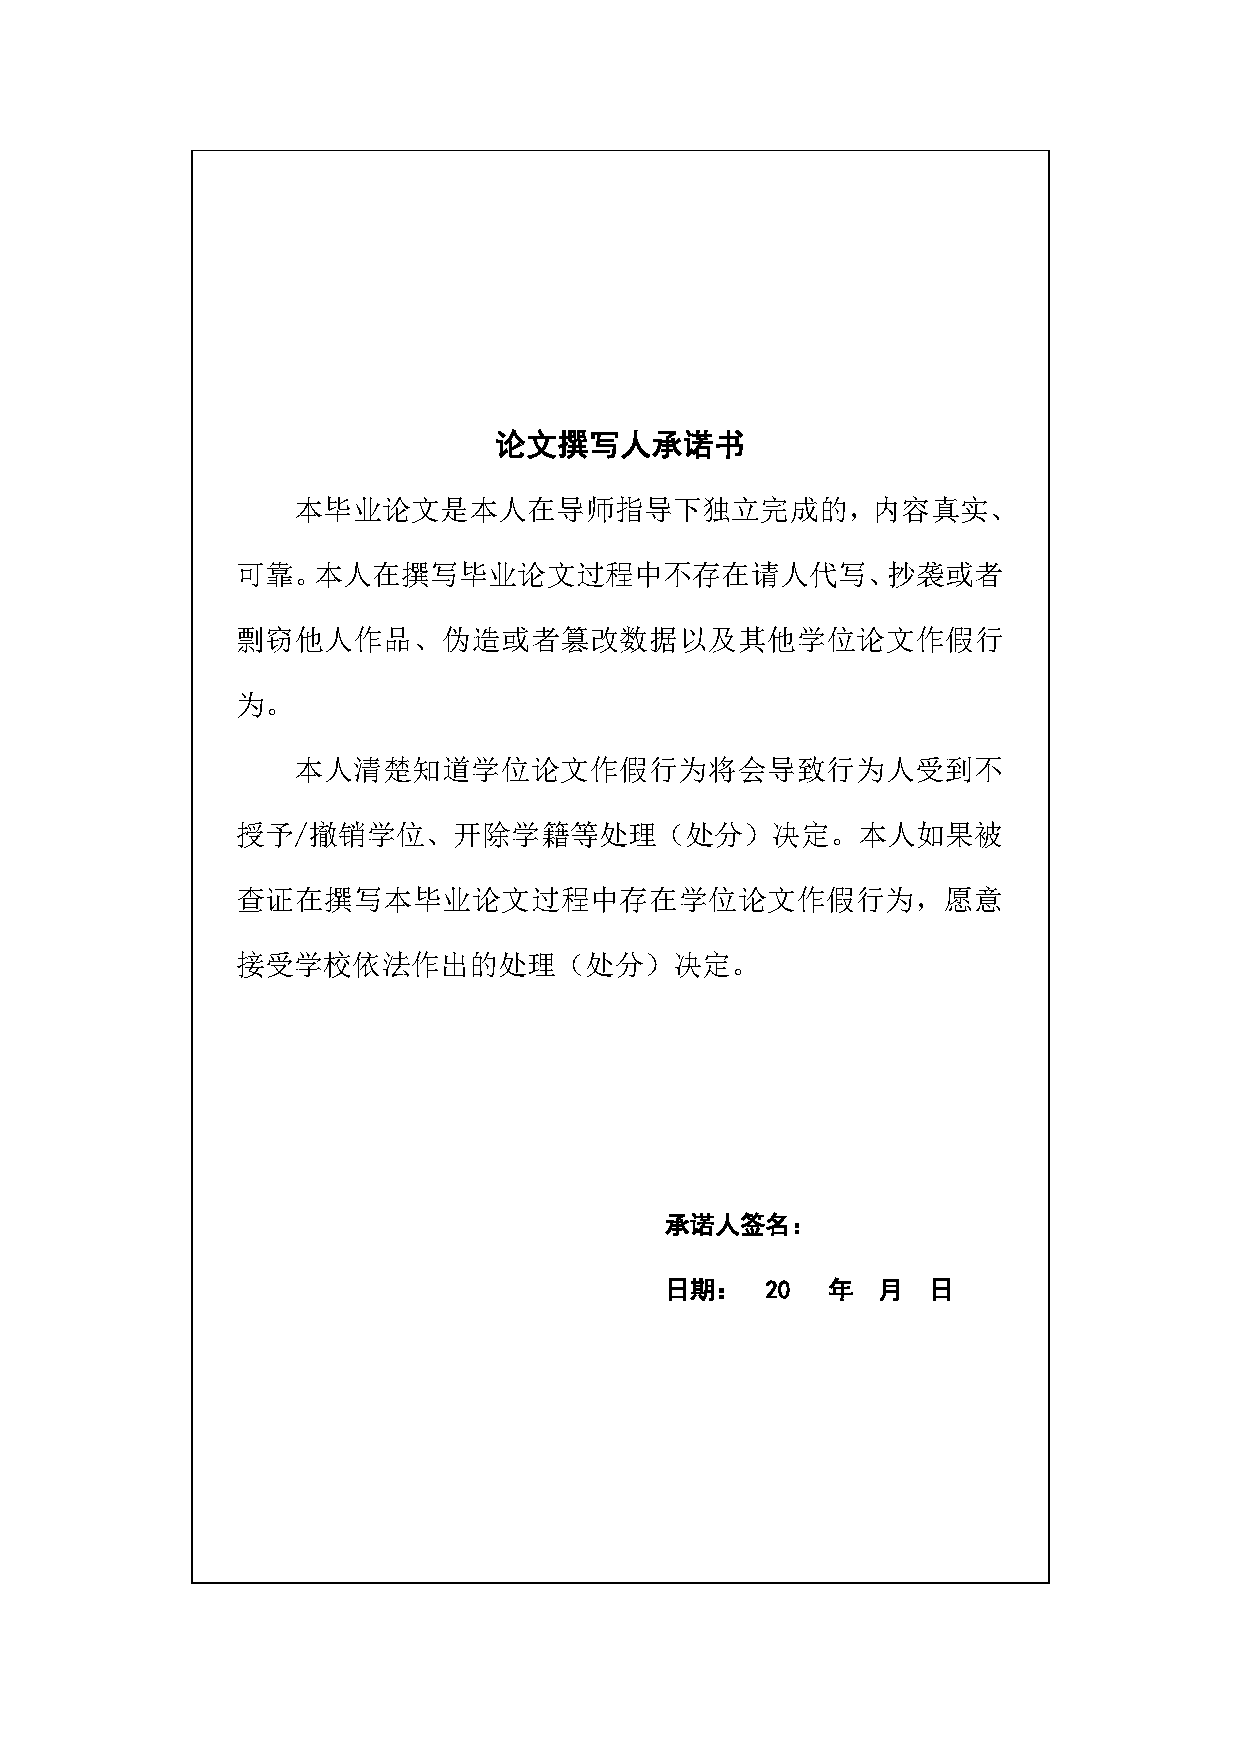
\includepdf[pages={1}]{coverii.pdf}}
% \renewcommand{\makecoveriii}{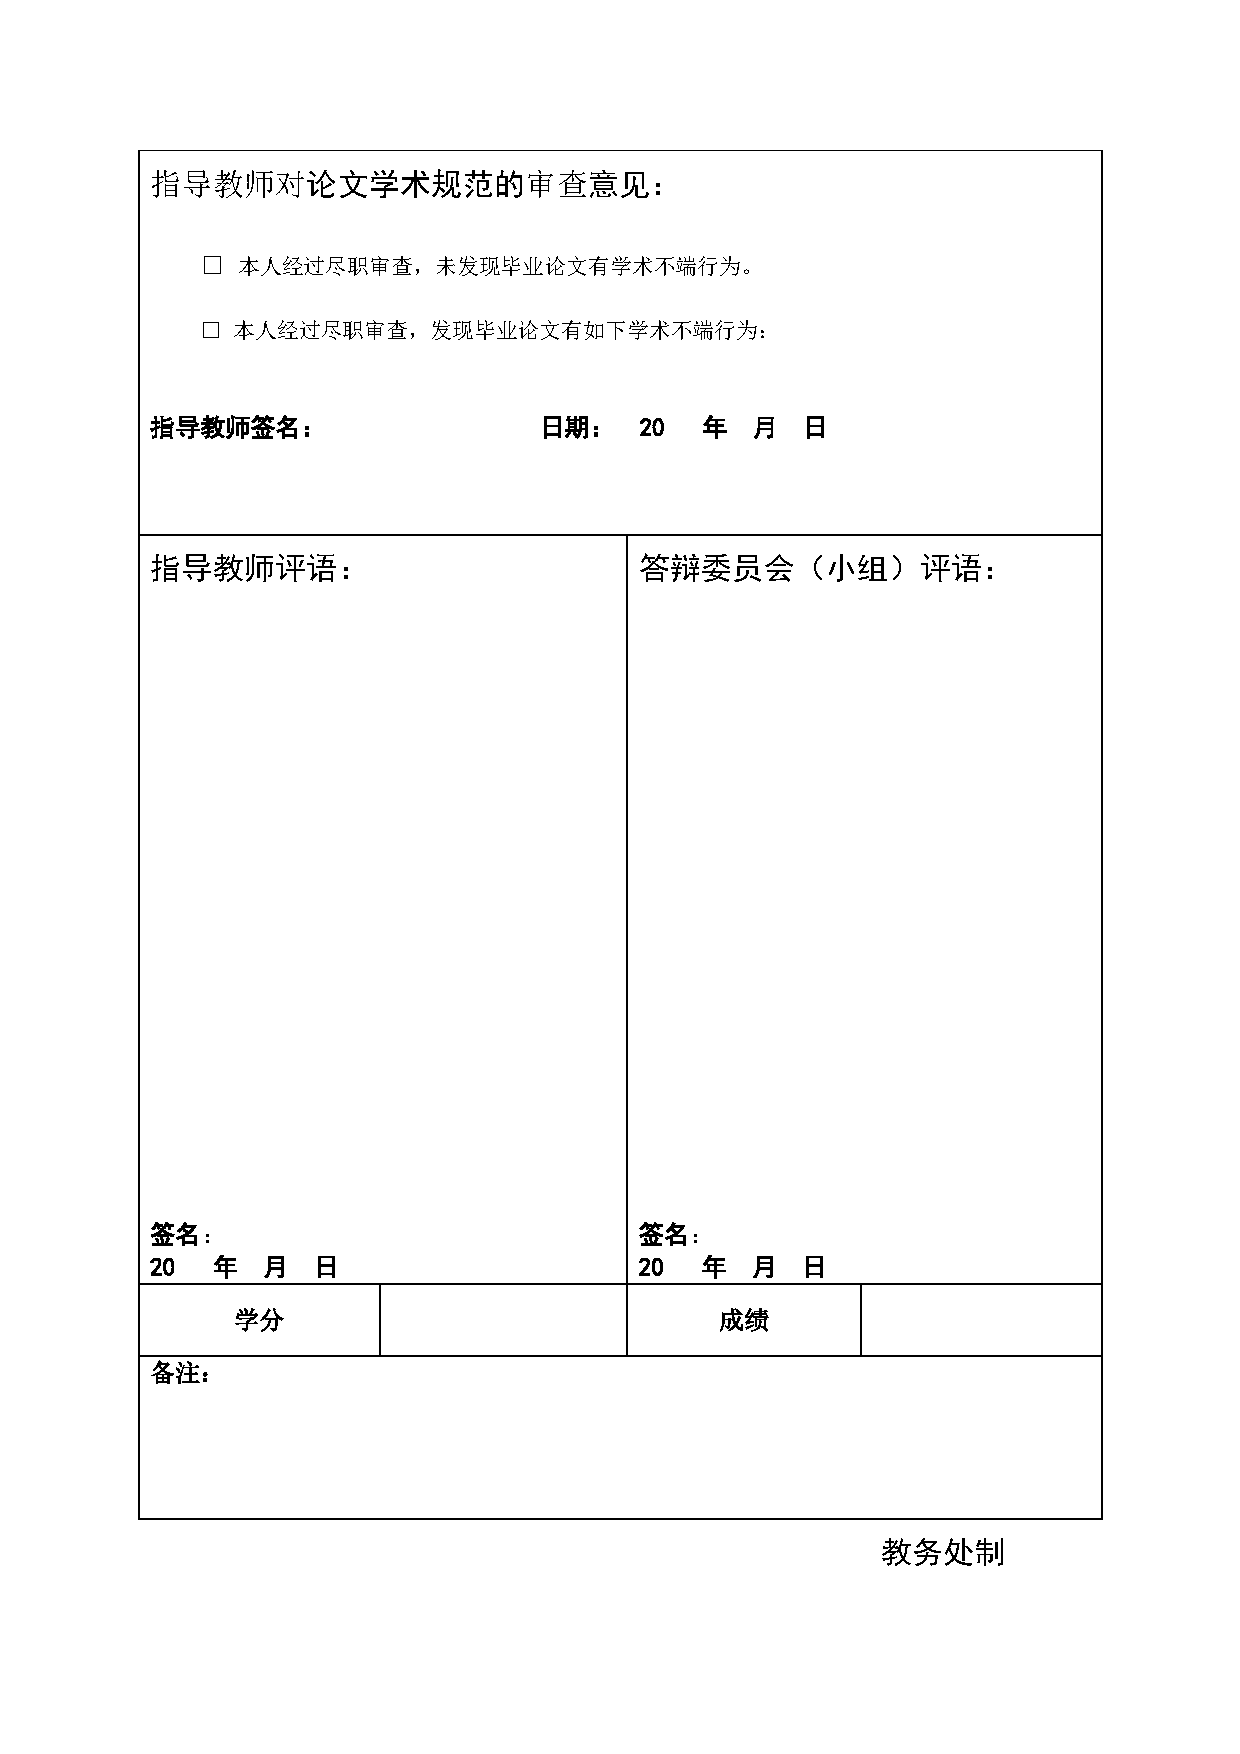
\includepdf[pages={1}]{coveriii.pdf}}

\begin{document}
  \frontmatter
    \begin{abstract}
      这是摘要.
    \end{abstract}

    \begin{abstract*}
      This is abstract.
    \end{abstract*}

    % \maketitle
    \tableofcontents

  \mainmatter
    \chapter{这是章}
      \section{这是节}
        \subsection{这是小节}
          这是正文.
          $$
            f(x)=\int_{\Omega}\mathscr{A}f(g)\,\mathrm{d}\mu(\omega)
          $$
          \newpage
          这是第二页的正文.
          \begin{proof}
            Proof Ends Here.
          \end{proof}

  \backmatter
    \begin{acknowledgement}
      这是致谢.
    \end{acknowledgement}

    \phantomsection\addcontentsline{toc}{chapter}{\textbf{参考文献}}
      \bibliographystyle{unsrt}
      \bibliography{test}
\end{document} 